\documentclass[12pt,a4paper]{article}
\usepackage{amsmath,amscd,amsbsy,amssymb,latexsym,url,bm,amsthm}
\usepackage{epsfig,graphicx,subfigure}
\usepackage{enumitem,balance}
\usepackage{wrapfig}
\usepackage{mathrsfs,euscript}
\usepackage[usenames]{xcolor}
\usepackage{hyperref}
\usepackage[vlined,ruled,linesnumbered]{algorithm2e}
\usepackage{array}
\hypersetup{colorlinks=true,linkcolor=black}
\usepackage{attachfile}
\usepackage{listings}
\usepackage{tabularx}

\newtheorem{theorem}{Theorem}
\newtheorem{lemma}[theorem]{Lemma}
\newtheorem{proposition}[theorem]{Proposition}
\newtheorem{corollary}[theorem]{Corollary}
\newtheorem{exercise}{Exercise}
\newtheorem*{solution}{Solution}
\newtheorem{definition}{Definition}
\theoremstyle{definition}

\renewcommand{\thefootnote}{\fnsymbol{footnote}}

\newcommand{\postscript}[2]
 {\setlength{\epsfxsize}{#2\hsize}
  \centerline{\epsfbox{#1}}}

\renewcommand{\baselinestretch}{1.0}

\setlength{\oddsidemargin}{-0.365in}
\setlength{\evensidemargin}{-0.365in}
\setlength{\topmargin}{-0.3in}
\setlength{\headheight}{0in}
\setlength{\headsep}{0in}
\setlength{\textheight}{10.1in}
\setlength{\textwidth}{7in}
\makeatletter \renewenvironment{proof}[1][Proof] {\par\pushQED{\qed}\normalfont\topsep6\p@\@plus6\p@\relax\trivlist\item[\hskip\labelsep\bfseries#1\@addpunct{.}]\ignorespaces}{\popQED\endtrivlist\@endpefalse} \makeatother
\makeatletter
\renewenvironment{solution}[1][Solution] {\par\pushQED{\qed}\normalfont\topsep6\p@\@plus6\p@\relax\trivlist\item[\hskip\labelsep\bfseries#1\@addpunct{.}]\ignorespaces}{\popQED\endtrivlist\@endpefalse} \makeatother

\begin{document}
\noindent

%========================================================================
\noindent\framebox[\linewidth]{\shortstack[c]{
\Large{\textbf{Lab06-Linear Programming}}\vspace{1mm}\\
CS214-Algorithm and Complexity, Xiaofeng Gao, Spring 2021.}}
\begin{center}
\footnotesize{\color{red}$*$ If there is any problem, please contact TA Haolin Zhou.}

% Please write down your name, student id and email.
\footnotesize{\color{blue}$*$ Name: Renyang Guan  \quad Student ID: 519021911058 \quad Email: guanrenyang@sjtu.edu.cn}
\end{center}

\begin{enumerate}
    \item
    \textit{Hirschberg Algorithm.} Recall the \textbf{String Similarity} problem in class, in which we calculate the edit distance between two strings in a sequence alignment manner.
    \begin{enumerate}
    	\item
    	Implement the algorithm combining \textbf{dynamic programming} and \textbf{divide-and-conquer} strategy in C/C++. Analyze the time complexity of your algorithm. {\color{blue}(The template \emph{Code-SequenceAlignment.cpp} is attached on the course webpage)}.
    	
    	\item
    	Given $\alpha(x, y) = |ascii(x) - acsii(y)|$, where $ascii(c)$ is the ASCII code of character $c$, and $\delta=13$. Find the edit distance between the following two strings.
    	\begin{align*}
    		X[1..60]=&\ CMQHZZRIQOQJOCFPRWOUXXCEMYSWUJ\\
    		&\ TAQBKAJIETSJPWUPMZLNLOMOZNLTLQ	
    	\end{align*}
    	\begin{align*}
    		Y[1..50]=&\ SUYLVMUSDROFBXUDCOHAATBKN\\
    		&\ AAENXEVWNLMYUQRPEOCJOCIMZ
    	\end{align*}
    \end{enumerate}
    \begin{solution}
    ~\\
    \begin{enumerate}
        \item [(a)] The algorithm is implemented in file Code-SequenceAlignment.cpp.
        \\
        \textbf{\textit{Time complexity analysis:}}
        \\
        The time complexity is $O(mn)$.
        \begin{proof}
        We could prove the conclusion by induction. Let $T(m,n)$ denotes the worst case time complexity. Suppose that $T(m,n)\leq kmn$, where $k$ is any positive integer. 
        \\
        \textbf{\textit{Basis step:}}
        When $m\leq 2$ and $n\leq 2$, the conclusion is obvious
        \\
        \textbf{\textit{Induction hypothesis:}} Suppose that for $m'$ and $n'$, where $m'n' < mn$ the hypothesis is true.
        \\
        \textbf{\textit{Proof of the induction step:}}
        We could generate such formula:
        \begin{equation}
            \begin{split}
                T(m,n) &\leq cmn+T(q,n/2)+T(m-q,n/2)\\
                       &\leq cmn+kqn/2+k(m-q)n/2\\
                       &=(c+k/2)mn
            \end{split}
        \end{equation}
        If $k=2c$ the conclusion is true.
        \end{proof}
        \item [(b)] The edit distance of the two strings is \textbf{385}.
    \end{enumerate}
    \end{solution}
    
    \item 
    \textit{Travelling Salesman Problem.} Given a list of cities and the distances between each pair of cities ($ G=(V,E,W) $), we want to find the shortest possible route that visits each city exactly once and returns to the origin city. Similar to \textbf{Maximum Independent Set} and \textbf{Dominating Set}, please turn the traveling salesman problem into an ILP form.  
    
    \textbf{Remark:} $ W $ is the set of weights corresponds to the edges that connecting adjacent cities.  
    \begin{solution}
    Suppose that $x_{uv}$ is a 0-1 indicator of the directed edge connecting vertex $u$ and $v$, such that:
    \begin{equation}\nonumber
        x_{uv}=
        \begin{cases}
        1 & the\ salesman\ does\ travel\ from\ u\ to\ v\ directly \\
        0 & the\ salesman\ does\ not\ travel\ from\ u\ to\ v\ directly
        \end{cases}
    \end{equation}
    Then $w_{uv}$ denotes the weight of the directed edge from vertex $u$ to $v$.
    Thus we can formulate the following ILP:
    \begin{equation}\nonumber
        \begin{split}
            & Goal:  \sum\limits_{u,v\in V} w_{uv}x_{uv}\\
            & s.t.\  \sum\limits_{v\in N(u)} x_{uv}=1\ \ \forall\ u\in V\\
            & \ \ \ \ \ \sum\limits_{v\in N(u)} x_{vu}=1\ \ \forall\ u \in V\\
            & \ \ \ \ \ \sum\limits_{u,v \in U}x_{uv}<|U|\ \forall\ U\subset V
        \end{split}
    \end{equation}
    where $N(u)$ denotes the set of neighbors of vertex $u$.
    \end{solution}
    
    
    \item
    \textit{Investment Strategy.} A company intends to invest $0.3$ million yuan in $2021$, with a proper combination of the following $3$ projects:
    \begin{itemize}
    \item \textbf{Project 1:} Invest at the beginning of a year, and can receive a $20\%$ profit of the investment in this project at the end of this year. Both the capital and profit can be invested at the beginning of next year;
    \item \textbf{Project 2:} Invest at the beginning of $2021$, and can receive a $50\%$ profit of the investment in this project at the end of $2022$. The investment in this project cannot exceed $0.15$ million dollars;
    \item \textbf{Project 3:} Invest at the beginning of $2022$, and can receive a $40\%$ profit of the investment in this project at the end of $2022$. The investment in this project cannot exceed $0.1$ million dollars.
    \end{itemize}
    Assume that the company will invest \emph{all} its money at the beginning of a year. Please design a scheme of investment in $2021$ and $2022$ which maximizes the overall sum of capital and profit at the end of $2022$.
    \begin{enumerate}
    \item
    Formulate a linear programming with necessary explanations.

    \item
    Transform your LP into its standard form and slack form.

    \item
    Transform your LP into its dual form.

    \item
    Use the simplex method to solve your LP.
    \end{enumerate}
    \begin{solution}
    ~\\
    \begin{enumerate}
        \item [(a)] 
        Suppose that $a_1$ and $a_2$ denote the investment of \emph{Project 1} in $2021$ and $2022$ respectively, $b$ denotes the investment of \emph{Project 2}, and $c$ denotes the investment of \emph{Project 3}.
        
        We can formulate the linear programming as follows:
        \begin{equation}\nonumber
            \begin{split}
             Goal: & max\ (120\% a_2+150\% b+140\% c) \\ 
             s.t.\  & a_1+b=0.3 \\
                    & a_2+c=120\% a_1\\ 
                    & b\leq 0.15\\
                    & c\leq 0.1 \\
                    & a_1,a_2,b,c\geq 0
            \end{split}
        \end{equation}
        \textit{Necessary explanation:} 
        \\
        At the beginning of $2021$, only \emph{Project 1} and \emph{Project 2} could be invested and all its money must be invested, such that equation $a_1+b=0.3$ holds. The money that can be invested at the end of $2022$ is the profit of $2021$, where the former is denoted as $a_2+c$ and the later is $120\% a_1$. Thus the equation $a_2+c=120\% a_1$ holds. The last two constraints are the requirement of \emph{Project 2} and \emph{Project 3} respectively.
        
        \item [(b)]
        \textbf{\textit{Standard form:}}
        \begin{equation}\nonumber
            \begin{split}
            Goal: & max\ (120\% a_2+150\% b+140\% c) \\ 
            s.t.\  & a_1+b\leq 0.3 \\
                    & -a_1-b\leq -0.3 \\
                    & a_2+c-120\% a_1\leq 0\\
                    & -a_2-c+120\% a_1\leq 0\\
                    & b\leq 0.15\\
                    & c\leq 0.1 \\
                    & a_1,a_2,b,c\geq 0
            \end{split}
        \end{equation}
        
        \textbf{\textit{Slack form:}}
        \begin{equation}\nonumber
            \begin{split}
             Goal: & max\ (120\% a_2+150\% b+140\% c) \\ 
             s.t.\  & a_1+b=0.3 \\
                    & a_2+c=120\% a_1\\ 
                    & b+x_1= 0.15\\
                    & c+x_2= 0.1 \\
                    & a_1,a_2,b,c\geq 0
            \end{split}
        \end{equation}
        $x_1$ and $x_2$ are slack variables.
        
        \item [(c)]
        \textbf{\textit{Dual form:}}
        \begin{equation}\nonumber
            \begin{split}
             Goal: & min\ (0.3y_1-0.3y_2+0.15y_5+0.1y_6) \\ 
             s.t.\  & y_1-y_2-120\%y_3+120\%y_4 \geq 0\\
                    & y_3-y_4\geq 120\% \\
                    & y_1-y_2+y_5\geq 150\% \\
                    & y_3-y_4+y_6\geq 140\% \\
                    & y_1,y_2,y_3,y_4,y_5,y_6 \geq 0
            \end{split}
        \end{equation}
        
        \item [(d)]
        \textbf{Step.1} Converting the LP into slack form which could be solved by simplex method. To do this, we must combine the two equations firstly:
        \begin{equation}
            \begin{cases}
            & a_1+b=0.3 \\
            & a_2+c=1.2 a_1\\ 
            \end{cases}
            \Rightarrow
            a_2+1.2b+c=0.36       
        \end{equation}
        and then bring the result int our goal, such that we have the slack form LP:
        \begin{equation}
            \begin{split}
                Goal: & max\ (0.06b+0.2c+0.432) \\ 
             s.t.\  & 0.15-b=x_1\\
                    & 0.1-c=x_2\\
                    & b,c,x_1,x_2\geq 0
            \end{split}
        \end{equation}
        \\
        \textbf{Step.2} Obtaining basic solution. In the question, the basic solution is 
        $$\Bar{X}=(\Bar{b},\Bar{c},\Bar{x_1},\Bar{x_2})=(0,0,0.15,0.1)$$
        \\
        \textbf{Step.3} Selecting nonbasic variable $b$.Since the \emph{tighter} constraint for $b$ is $0.15-b=x_1$, we change it into $0.15-x_1=b$
        \textbf{Step.4} Pivoting
        \\
        Currently the LP is transformed as:
        \begin{equation}\nonumber
            \begin{split}
             Goal: & max\ (-0.06x_1+0.2c+0.441) \\ 
             s.t.\  & 0.15-x_1=b\\
                    & 0.1-c=x_2\\
                    & b,c,x_1,x_2\geq 0
            \end{split}
        \end{equation}
        \textbf{Step.5} Repeat Step2 to Step4
        The final form of primitive LP is 
        \begin{equation}\nonumber
            \begin{split}
             Goal: & max\ (-0.06x_1-0.2x_2+0.461) \\ 
             s.t.\  & 0.15-x_1=b\\
                    & 0.1-x_2=c\\
                    & b,c,x_1,x_2\geq 0
            \end{split}
        \end{equation}
        
        \textbf{\textit{Final solution:}} 
        $$\Bar{x}=(0.15,0.1,0,0)$$
        and the goal is \textbf{0.461}.
    \end{enumerate}
    \end{solution}
    \item
    \textit{Factory Production.} An engineering factory makes seven products (PROD 1 to PROD 7) on the following machines: four grinders, two vertical drills, three horizontal drills, one borer and one planer. Each product yields a certain contribution to profit (in \pounds/unit). These quantities (in \pounds/unit) together with the unit production times (hours) required on each process are given below. A dash indicates that a product does not require a process.

    \begin{table}[htbp]
      \scriptsize
      \centering
      \renewcommand\arraystretch{1.1}
      \begin{tabular}{m{0.18\textwidth} m{0.07\textwidth}<{\centering} m{0.07\textwidth}<{\centering} m{0.07\textwidth}<{\centering} m{0.07\textwidth}<{\centering} m{0.07\textwidth}<{\centering} m{0.07\textwidth}<{\centering} m{0.07\textwidth}<{\centering}}
      \hline
       & \textbf{PROD 1} & \textbf{PROD 2} & \textbf{PROD 3} & \textbf{PROD 4} & \textbf{PROD 5} & \textbf{PROD 6} &  \textbf{PROD 7} \\\hline
      Contribution to profit & 10 & 6 & 8 & 4 & 11 & 9 & 3 \\
      Grinding & 0.5 & 0.7 & - & - & 0.3 & 0.2 & 0.5 \\
      Vertical drilling & 0.1 & 0.2 & - & 0.3 & - & 0.6 & - \\
      Horizontal drilling & 0.2 & - & 0.8 & - & - & - & 0.6 \\
      Boring & 0.05 & 0.03 & - & 0.07 & 0.1 & - & 0.08 \\
      Planing & - & - & 0.01 & - & 0.05 & - & 0.05 \\
      \hline
      \end{tabular}
    \end{table}

    There are marketing limitations on each product in each month, given in the following table:

    \begin{table}[htbp]
      \scriptsize
      \centering
      \renewcommand\arraystretch{1.1}
      \begin{tabular}{m{0.1\textwidth} m{0.07\textwidth}<{\centering} m{0.07\textwidth}<{\centering} m{0.07\textwidth}<{\centering} m{0.07\textwidth}<{\centering} m{0.07\textwidth}<{\centering} m{0.07\textwidth}<{\centering} m{0.07\textwidth}<{\centering}}
      \hline
       & \textbf{PROD 1} & \textbf{PROD 2} & \textbf{PROD 3} & \textbf{PROD 4} & \textbf{PROD 5} & \textbf{PROD 6} &  \textbf{PROD 7} \\\hline
      January & 500 & 1000 & 300 & 300 & 800 & 200 & 100 \\
      February & 600 & 500 & 200 & 0 & 400 & 300 & 150 \\
      March & 300 & 600 & 0 & 0 & 500 & 400 & 100 \\
      April & 200 & 300 & 400 & 500 & 200 & 0 & 100 \\
      May & 0 & 100 & 500 & 100 & 1000 & 300 & 0 \\
      June & 500 & 500 & 100 & 300 & 1100 & 500 & 60 \\
      \hline
      \end{tabular}
    \end{table}

    It is possible to store up to 100 of each product at a time at a cost of \pounds0.5 per unit per month (charged at the end of each month according to the amount held at that time). There are no stocks at present, but it is desired to have a stock of exactly 50 of each type of product at the end of June. The factory works six days a week with two shifts of 8h each day. It may be assumed that each month consists of only 24 working days. Each machine must be down for maintenance in one month of the six. No sequencing problems need to be considered.

    When and what should the factory make in order to maximize the total net profit?

    \begin{enumerate}
    \item
    Use \emph{CPLEX Optimization Studio} to solve this problem. Describe your model in \emph{Optimization Programming Language} (OPL). Remember to use a separate data file (.dat) rather than embedding the data into the model file (.mod).

    \item
    Solve your model and give the following results.
    \begin{enumerate}
    \item
    For each machine:
    \begin{enumerate}
    \item
    the month for maintenance.
    \end{enumerate}
    \item
    For each product:
    \begin{enumerate}
    \item
    The amount to make in each month.
    
    \item
    The amount to sell in each month.
    \item
    The amount to hold at the end of each month.
    \end{enumerate}
    \item
    The total selling profit.
    \item
    The total holding cost.
    \item
    The total net profit (selling profit minus holding cost).
    \end{enumerate}
    \end{enumerate}
    \textbf{Remark:} You can choose to use the attached .dat file or write it yourself. 
    
    \textbf{\textit{Model:}} The linear programming model is described in file \emph{FactoryPlanning.mod}.
    \\
    \textbf{\textit{Results:}} The results are shown in , respectively.
    \begin{enumerate}
        \item [i.] The result is shown in Fig.~\ref{Fig-Stop}. The number in the table illustrate the number of machines which are down for maintenance in each particular month.
        
        \item [ii.]
        \begin{enumerate}
            \item [A.] is shown in Fig.~\ref{Fig-Produce}.
            \item [B.] is shown in Fig.~\ref{Fig-Sell}.
            \item [C.] is shown in Fig.~\ref{Fig-Hold}.
            \begin{figure}[htbp]
            \centering 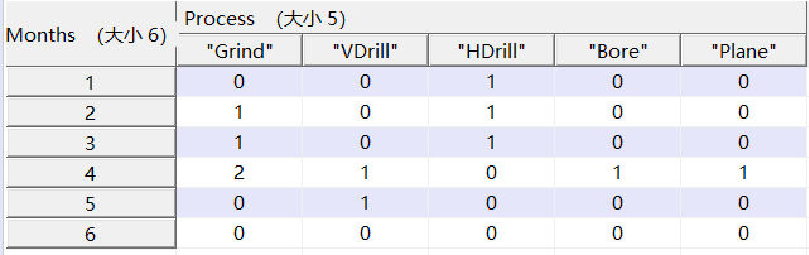
\includegraphics[width=0.8\textwidth]{Fig-Stop.pdf}
            \caption{The month for maintenance}\label{Fig-Stop}
            \end{figure}
            \begin{figure}[htbp]
            \centering 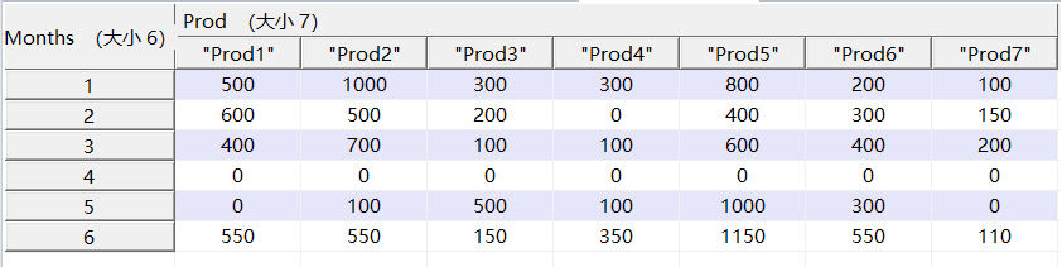
\includegraphics[width=0.8\textwidth]{Fig-Produce.pdf}
            \caption{The amount to make in each month}\label{Fig-Produce}
            \end{figure}
            
            
            \begin{figure}[htbp]
            \centering 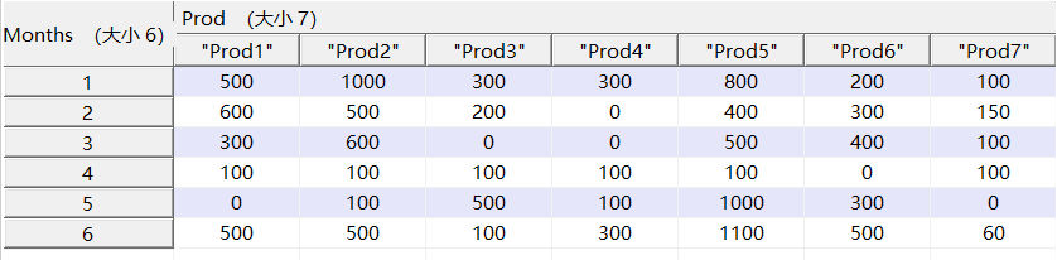
\includegraphics[width=0.8\textwidth]{Fig-Sell.pdf}
            \caption{The amount to sell in each month}\label{Fig-Sell}
            \end{figure}
            
            \begin{figure}[htbp]
            \centering 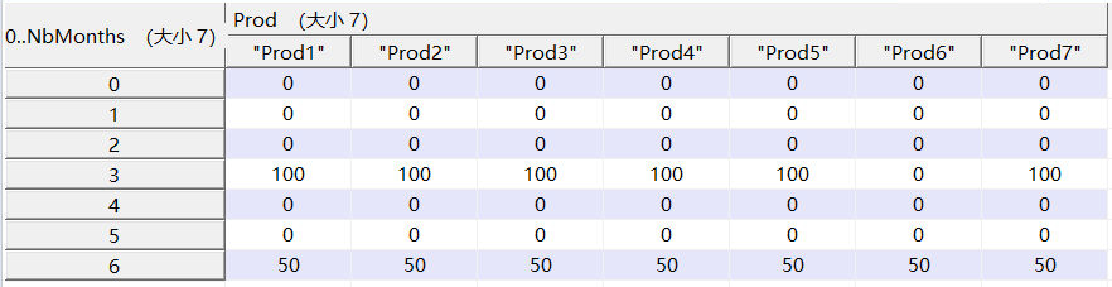
\includegraphics[width=0.8\textwidth]{Fig-Hold.pdf}
            \caption{The amount to hold at the end of each month}\label{Fig-Hold}
            \end{figure}
            
        \end{enumerate}
        \item [iii.] The total selling profit is \textbf{109330}.
        \item [iv.]  The total holding cost is \textbf{475}.
        \item [v.]   The total net profit is \textbf{108855}.
    \end{enumerate}
    
    
\end{enumerate}
\newpage
\vspace{20pt}

{\noindent\large\textbf{Appendix}}
\begin{enumerate}
	\item [\textbf{A.}]
	\textbf{FactoryPlanning.dat}
	\attachfile{FactoryPlanning.dat}
	\lstset{
		language=C,
		tabsize=2,
		basicstyle=\footnotesize\ttfamily,
		columns=fullflexible,
		keywordstyle=\color{blue},
		numbers=left,
		numberstyle=\scriptsize\ttfamily,
		frame=single
	}
	\begin{lstlisting}
		NbMonths = 6;
		
		Prod = {Prod1, Prod2, Prod3, Prod4, Prod5, Prod6, Prod7};
		Process = {Grind, VDrill, HDrill, Bore, Plane};
		
		// profitProd[j] is profit per unit for product j
		ProfitProd = [10 6 8 4 11 9 3];
		
		// processProd[i][j] gives hours of process i required by product j
		ProcessProd = [[0.5  0.7  0.0  0.0  0.3  0.2 0.5 ]
		[0.1  0.2  0.0  0.3  0.0  0.6 0.0 ]
		[0.2  0.0  0.8  0.0  0.0  0.0 0.6 ]
		[0.05 0.03 0.0  0.07 0.1  0.0 0.08]
		[0.0  0.0  0.01 0.0  0.05 0.0 0.05]];
		
		// marketProd[i][j] gives marketing limitation on product j for month i
		MarketProd = [[500 1000 300  300 800  200 100]
		[600 500  200  0   400  300 150]
		[300 600  0    0   500  400 100]
		[200 300  400  500 200  0   100]
		[0   100  500  100 1000 300 0  ]
		[500 500  100  300 1100 500 60 ]];
		
		CostHold  = 0.5;
		StartHold = 0;
		EndHold   = 50;
		MaxHold   = 100;
		
		// process capacity
		HoursMonth = 384; // 2 eight hour shifts per day, 24 working days per month;
		
		// number of each type of machine
		NumProcess = [4 2 3 1 1];
		
		// how many machines must be down over 6 month period
		NumDown = [4 2 3 1 1];
	\end{lstlisting}
\end{enumerate}

\textbf{Remark:} You need to include your .cpp, .mod, .dat, .pdf and .tex files in your uploaded .zip file.

%========================================================================
\end{document}
